\documentclass[11pt,twocolumn]{article}

\usepackage[a4paper,margin=18mm,columnsep=7mm]{geometry}
\usepackage{amsmath}
\usepackage{array}
\usepackage{booktabs}
\usepackage{graphicx}
\usepackage{microtype}
\usepackage{tikz}
\usepackage{url}
\usepackage[hidelinks]{hyperref}
\usepackage{xcolor}
\usetikzlibrary{arrows.meta,fit,positioning,shapes.geometric,patterns}

\hypersetup{
  pdftitle={RV565: Cross-Layer Co-Design for Frame-Independent Video Playback on MicroPython-Class ESP32-S3 Systems},
  pdfauthor={Ayushman Bhattacharya, Anwesha Chakraborty},
  pdfsubject={Compressed RGB565 media playback on an ESP32-S3 application platform},
  pdfkeywords={RV565, ESP32-S3, RGB565, MicroPython, DMA, embedded video, Deflate, SPI display}
}

\newcommand{\system}{RV565}
% Set to the Zenodo DOI of the archived artifact before submission.
\newcommand{\artifactdoi}{10.5281/zenodo.XXXXXXX}

\title{\system: Cross-Layer Co-Design for Frame-Independent\\
Video Playback on MicroPython-Class ESP32-S3 Systems}
\author{Ayushman Bhattacharya\textsuperscript{1} \quad
Anwesha Chakraborty\textsuperscript{2}\\[-0.15em]
{\small \textsuperscript{1}Pollinations AI \quad
\textsuperscript{2}Department of Computer Science and Engineering, JIS University}\\[-0.15em]
{\scriptsize \texttt{ayushman.elixpo@gmail.com} \quad
\texttt{anwesha.elixpo@gmail.com}}}
\date{}

\begin{document}
\maketitle

\begin{abstract}
Video on SPI-attached microcontroller displays is limited less by decoding
than by where each byte lives and which stages run serially.  We present
\system, a frame-independent video container whose decoded representation is
the panel's native RGB565 format, and use it to characterise two data paths on
an ESP32-S3: a standalone firmware that overlaps nearest-neighbour scaling with
SPI direct-memory-access (DMA) transfers through two internal-memory stripes,
and the same media played inside OreoOS, a MicroPython application operating
system.  Across ten runs and 7,200 frames, the standalone path sustains
24.004~FPS with no drop or deadline miss; its display transfer runs at 98.1\%
of the 40~MHz wire-time bound while the CPU is idle for 90.9\% of it.  The
integrated path reaches 14.093~FPS; stage timing attributes its 69.2~ms mean
frame time to serialized filesystem input, inflation, scaling into an
external-RAM framebuffer, and blocking presentation, with only 0.8~ms of
interpreter overhead.  Two further results follow from the measurements.
First, per-frame inflation time is linear in the compressed length stored in
the container ($r^2=0.957$; 0.14~ms mean error on held-out frames), so decode
cost can be bounded before playback.  Second, frame independence costs only
0.6--1.7\% in size relative to a single Deflate stream, because a 48.6~KB
RGB565 frame exceeds Deflate's 32~KiB match window; we derive the general
condition.  Firmware, media hashes, raw logs, and analysis scripts are
released.
\end{abstract}

\section{Introduction}

Video playback on a microcontroller is not solely a decoding problem.  A
complete frame must be fetched, decoded, transformed to the panel's pixel
layout, and transferred before its presentation deadline.  At the same time,
an interactive device must continue polling buttons and servicing operating
system work.  These constraints are especially visible on SPI-connected
displays, for which transfer time consumes a substantial and predictable part
of every frame period.

General-purpose video formats optimise compression ratio, interoperability,
and visual quality.  They commonly introduce container parsing, colour-space
conversion, variable decoder state, and inter-frame dependencies.  Those
features are valuable on larger systems, but can make latency and memory use
difficult to bound on a microcontroller.  Raw RGB565 has the opposite
trade-off: display transfer is simple and deterministic, while storage and
input bandwidth scale directly with the number of pixels.

Existing approaches can be organised along three architectural axes.  The
first is \emph{where decode complexity resides}: display-native raw
playback~\cite{microchip2012video} moves all work to the host and pays in
storage, whereas transform codecs such as JPEG~\cite{wallace1991jpeg} and its
embedded decoders~\cite{chan2021tjpgd,espressif2026newjpeg} place inverse
transforms and colour conversion on the device.  The second is
\emph{inter-frame dependence}: motion-compensated codecs such as
H.264/AVC~\cite{wiegand2003overview} reach high compression through reference
pictures, while intra-only streams such as MJPEG decode every frame in
isolation; software decoders for dependent streams on general-purpose
processors~\cite{lee1995realtime} and media processors~\cite{mattavelli1998implementing}
had to predict and schedule variable decode complexity to stay real-time.
The third is \emph{the distance between the decoded format and the panel
format}: decoders that emit RGB888 or YUV require a conversion pass before an
RGB565 panel can be driven, while byte-oriented lossless formats such as
QOI~\cite{szablewski2022qoi} and LZ4~\cite{collet2024lz4} trade compression
ratio for decode speed but are not tied to a display format.  Integrated
frameworks~\cite{espressif2026player} span several of these points.  On a
microcontroller, each axis maps onto a hardware resource: device decode work
consumes CPU cycles during the frame period, inter-frame state consumes
scarce internal SRAM, and format conversion adds a full pass over the frame
through the memory hierarchy.

\system{} occupies a deliberately narrow point in this space: host-side
resampling and colour quantisation, intra-only frames, and lossless Deflate
payloads~\cite{deutsch1996deflate} whose decoded bytes are already the panel's
RGB565 format.  This work asks where the frame budget actually goes for such a
stream on an ESP32-S3, both on bare firmware and inside
OreoOS~\cite{bhattacharya2026oreo}, a MicroPython~\cite{micropython}
application operating system.  We do not propose a new entropy coder; the
contribution is the co-design of representation, memory placement,
scheduling, and display I/O, and an architectural characterisation that
explains its behaviour.

Our contributions to the study of embedded media architectures are as
follows.  We define a frame-independent, display-native container with a
host- and device-side validation contract
(Sections~\ref{sec:container}--\ref{sec:validation}).  We build a standalone
data path in which double-buffered internal-SRAM stripes overlap scaling with
SPI direct-memory-access (DMA) transfers, sustaining 24.004~FPS with zero
deadline misses and placing the display transfer within 1.9\% of the
wire-time bound, which shows that this class of system is bus-bound rather
than decode-bound (Section~\ref{sec:bus}).  We show that intra-only Deflate
makes decode cost a linear function of the payload length already stored in
the container, so the complexity prediction that earlier real-time decoders
had to estimate~\cite{mattavelli1998implementing} becomes available from
metadata before playback (Section~\ref{sec:model}).  We quantify the storage
cost of frame independence at 0.6--1.7\% and derive the condition under which
Deflate's match window cannot exploit co-located temporal redundancy at all
(Section~\ref{sec:independence}).  Finally, we provide a stage-resolved
characterisation of interpreter-hosted playback showing that the gap between
bare firmware and an application OS is caused by serialization and memory
placement rather than interpreter overhead (Section~\ref{sec:gap}).  All
firmware, measurements, and analysis scripts are
public~\cite{bhattacharya2026oreo}.

\section{RGB565 as the Design Starting Point}

RGB565 encodes one pixel in 16 bits: five bits represent red, six represent
green, and five represent blue.  Green receives the additional bit because
human vision is comparatively sensitive to luminance detail in that portion
of the spectrum.  A pixel can be written as

\begin{equation}
p=(r_5 \ll 11)\;|\;(g_6 \ll 5)\;|\;b_5,
\label{eq:pixel}
\end{equation}

where $r_5$, $g_6$, and $b_5$ are quantised colour components.  \system{}
stores the 16-bit value of Eq.~\eqref{eq:pixel} in the big-endian byte order
that the panel controller expects on its serial interface, so a decoded frame
can move toward the display without an intermediate RGB888 or YUV conversion.

This choice simplifies the device but exposes the system constraint.  A frame
contains $W\times H$ pixels and therefore occupies

\begin{equation}
B_{frame}=2WH
\label{eq:frame}
\end{equation}

bytes before compression (Eq.~\eqref{eq:frame}).  Frame rate multiplies that value into a continuous
storage and memory-bandwidth demand, while the final 320$\times$240 image must
still cross the SPI bus.  \system{} consequently compresses what is stored and
read, not what the display ultimately receives.  Every successfully decoded
frame has a deterministic size and colour layout, which keeps validation,
scaling, and presentation straightforward.

RGB565 also defines the quality boundary.  Deflate is lossless with respect to
the encoded bytes, but conversion from the original colour space and spatial
resizing are not.  Any loss in \system{} therefore arises from resampling and
RGB565 quantisation, never from compression.  \system{} is a media
architecture built around a native pixel representation, not a claim that
16-bit colour is visually lossless relative to the source.

\section{From a Gallery Feature to a Systems Problem}

The project began with a modest goal: Gallery already displayed still images,
so video appeared to be a sequence of images plus a clock.  The first player
followed that model literally.  It read a frame, decoded it in MicroPython,
scaled pixels in Python loops, copied the result into the framebuffer, and
asked the normal display driver to present it.  The result was technically a
video player, but not an interactive one.  A frame occupied the interpreter
for so long that playback advanced visibly rather than continuously, and
button events waited behind media work.

That failure changed the question.  The problem was no longer how to parse a
video file; it was how to move one complete frame through storage, memory,
conversion, and the display bus before the next deadline while still returning
to the operating-system loop.  Each later version removed one bottleneck from
that path (Figure~\ref{fig:evolution}).  The intermediate prototypes were not
instrumented, so this history is qualitative; only \system{} v6 is evaluated
quantitatively.

\begin{figure*}[t]
\centering
\resizebox{0.96\textwidth}{!}{%
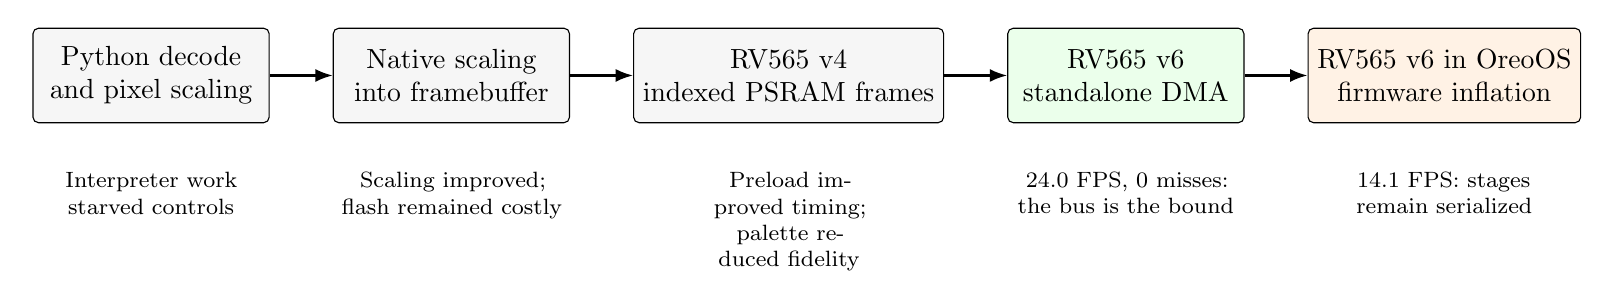
\begin{tikzpicture}[
  stage/.style={draw, rounded corners=2pt, minimum width=30mm,
                minimum height=12mm, align=center, fill=gray!7},
  lesson/.style={font=\footnotesize, align=center, text width=29mm},
  arrow/.style={-{Latex[length=2.2mm]}, thick},
  node distance=8mm
]
  \node[stage] (python) {Python decode\\and pixel scaling};
  \node[stage, right=of python] (native) {Native scaling\\into framebuffer};
  \node[stage, right=of native] (v4) {\system{} v4\\indexed PSRAM frames};
  \node[stage, right=of v4, fill=green!8] (standalone) {\system{} v6\\standalone DMA};
  \node[stage, right=of standalone, fill=orange!10] (os) {\system{} v6 in OreoOS\\firmware inflation};

  \draw[arrow] (python) -- (native);
  \draw[arrow] (native) -- (v4);
  \draw[arrow] (v4) -- (standalone);
  \draw[arrow] (standalone) -- (os);

  \node[lesson, below=5mm of python] {Interpreter work\\starved controls};
  \node[lesson, below=5mm of native] {Scaling improved;\\flash remained costly};
  \node[lesson, below=5mm of v4] {Preload improved timing;\\palette reduced fidelity};
  \node[lesson, below=5mm of standalone] {24.0 FPS, 0 misses:\\the bus is the bound};
  \node[lesson, below=5mm of os] {14.1 FPS: stages\\remain serialized};
\end{tikzpicture}}
\caption{\system{} evolved by following the bottleneck exposed by each
prototype.  The first three stages are qualitative history.  The two \system{}
v6 stages are measured in Section~\ref{sec:evaluation}; fusing the standalone
DMA path into OreoOS remains future work.}
\label{fig:evolution}
\end{figure*}

\subsection{Moving pixels out of Python}

The first correction was a native scaler that wrote RGB565 pixels directly
into the display framebuffer.  This removed nested Python loops and restored
much of the frame budget, but it also revealed the next cost: repeatedly
reading frame-sized payloads from the filesystem.  Optimising the computation
had merely exposed the storage path.

\system{} v4 responded by moving expensive colour analysis to the host.  Each
frame carried an adaptive RGB565 palette and an 8-bit index plane.  Gallery
loaded those independent frame blocks into PSRAM incrementally and the native
module expanded them directly into the output framebuffer.  Blocks were used
instead of one monolithic allocation because a long-running UI can have ample
total PSRAM yet lack one sufficiently large contiguous region.  The design
removed the per-frame filesystem read, but a per-frame palette placed an
avoidable ceiling on image fidelity.

\subsection{Separating the hardware limit from the OS cost}

\system{} v6 returned to full-colour RGB565 frames and compressed each one
independently.  To learn whether the hardware could sustain the intended
playback rate, we temporarily removed the operating system and built a
standalone ESP-IDF experiment that inflates frames natively and transfers
the scaled output through two internal-memory stripes with SPI2 GDMA.  It
sustains the 24~FPS target (Section~\ref{sec:standalone-results}).

Reintroducing the operating system made the remaining boundary visible.  We
moved Deflate decoding below the Python boundary into a firmware-resident
module, but kept Gallery's existing filesystem input, framebuffer scaling, and
display driver.  That integrated path reaches 14.093~FPS.  Rather than
treating the shortfall as interpreter overhead, Section~\ref{sec:gap}
decomposes it stage by stage.  This history matters to the method: the
architecture was derived by measuring and relocating the critical path one
layer at a time, and the measurements show which layer must move next.

\section{Background and Previous Work}

\system{} combines established ideas---display-native pixels, independent
compression, external memory, and DMA-backed transfers---under the constraints
of an interactive MicroPython system.  Table~\ref{tab:literature} compares the
approaches introduced above along the axes of the taxonomy; this section
discusses each family and separates its foundations from the contribution of
\system{}.

\begin{table*}[t]
\centering
\caption{Comparison of video and image representations relevant to
SPI-display microcontrollers, organised by the taxonomy of the introduction.
``Inter-frame state'' is decoder state carried between frames; ``device
work'' is the dominant per-frame operation on the decoding processor.}
\label{tab:literature}
\small
\setlength{\tabcolsep}{4pt}
\begin{tabular}{@{}>{\raggedright\arraybackslash}p{0.18\textwidth}%
                >{\raggedright\arraybackslash}p{0.18\textwidth}%
                >{\raggedright\arraybackslash}p{0.10\textwidth}%
                >{\raggedright\arraybackslash}p{0.18\textwidth}%
                >{\raggedright\arraybackslash}p{0.11\textwidth}%
                >{\raggedright\arraybackslash}p{0.14\textwidth}@{}}
\toprule
Approach & Representation & Inter-frame state & Device work per frame & Random access & Target platform \\
\midrule
Raw RGB565 playback~\cite{microchip2012video} & Uncompressed display-native frames & None & Copy to panel & Fixed offsets & PIC MCU \\
JPEG / TJpgDec~\cite{wallace1991jpeg,chan2021tjpgd} & Baseline JPEG; RGB565 output option & None & Huffman, IDCT, colour conversion & Per image & Low-memory MCU \\
ESP\_NEW\_JPEG~\cite{espressif2026newjpeg} & JPEG with SIMD acceleration & None & Huffman, IDCT, colour conversion & Per image & ESP32-S3 \\
ESP Player~\cite{espressif2026player} & MJPEG or H.264 in a container & H.264 only & Demux, decode, render, A/V sync & Container seek & Espressif SoCs \\
H.264/AVC~\cite{wiegand2003overview} & Motion-compensated transform coding & Reference pictures & Prediction, transform, filtering & From key frames & Hardware or large CPU \\
Software MPEG~\cite{lee1995realtime} & MPEG-1 & Reference pictures & Software decode with media instructions & From key frames & Workstation RISC CPU \\
Complexity prediction~\cite{mattavelli1998implementing} & MPEG with predicted decode cost & Reference pictures & Decode under a predicted schedule & From key frames & Media processor \\
QOI~\cite{szablewski2022qoi} & Byte-oriented lossless image & None & Run, index and delta ops & Per image & General \\
LZ4 frame~\cite{collet2024lz4} & LZ77 without entropy stage & Within stream & Byte-copy decoding & None in frame format & General \\
\midrule
\system{} v6 (this work) & Display-native RGB565, per-frame Deflate & None & Inflate; scaling overlapped with DMA & $O(1)$ via length index & ESP32-S3, bare or MicroPython \\
\bottomrule
\end{tabular}
\end{table*}

\subsection{Display-native playback}

Microcontroller video demonstrations have long stored frames in a form close
to the display representation.  Microchip's AN1415, for example, describes
RGB565 video playback from removable storage~\cite{microchip2012video}.  Such
designs minimise device-side transformation but trade storage capacity and
input bandwidth for simple execution.  \system{} retains a display-native
decoded frame while compressing each frame independently to reduce storage
and input traffic.

\subsection{Transform codecs and embedded decoders}

JPEG is a widely deployed still-image coding standard~\cite{wallace1991jpeg},
and concatenated JPEG images form a practical MJPEG stream.  TJpgDec is a
baseline JPEG decompressor designed for very small memory footprints, with an
RGB565 output option~\cite{chan2021tjpgd}; Espressif's ESP\_NEW\_JPEG library
uses the ESP32-S3's SIMD instructions to accelerate JPEG encoding and
decoding~\cite{espressif2026newjpeg}.  Espressif's multimedia framework
supports MJPEG and H.264 playback, demultiplexing, rendering, seeking, and
audio/video synchronisation~\cite{espressif2026player}, and is therefore an
important implementation baseline.  These decoders spend device cycles on
entropy decoding, inverse transforms, and colour conversion; \system{} moves
the transform and quantisation to the host and leaves only inflation.

\subsection{Inter-frame codecs and decode-cost prediction}

H.264/AVC achieves high compression with motion-compensated prediction from
reference pictures~\cite{wiegand2003overview}.  Software decoding of such
streams was first made real-time on general-purpose processors with media
instructions~\cite{lee1995realtime}.  Because the decode cost of dependent
frames varies with content and reference structure, Mattavelli et al.\
predicted per-frame complexity to schedule decoding on media
processors~\cite{mattavelli1998implementing}.  \system{} reaches the same
scheduling goal from the opposite direction: with intra-only, single-codec
frames, decode cost becomes a measured linear function of a length that the
container already stores (Section~\ref{sec:model}).

\subsection{Lossless compression and independent frames}

Deflate combines the dictionary construction introduced by Ziv and
Lempel~\cite{ziv1977universal} with Huffman's minimum-redundancy prefix
codes~\cite{huffman1952method}; RFC~1951 defines their use in the Deflate
bitstream, including a maximum back-reference distance of
32,768~bytes~\cite{deutsch1996deflate}.  The zlib wrapper specifies framing
and integrity metadata~\cite{deutsch1996zlib}.  Both \system{} decoders use
the \texttt{tinfl} inflater from miniz~\cite{miniz}, which the ESP32-S3 also
provides in ROM.  Faster byte-oriented alternatives exist: LZ4 omits the
entropy stage entirely~\cite{collet2024lz4}, and QOI encodes images with a
small set of run, index, and delta operations~\cite{szablewski2022qoi}.
\system{} uses Deflate because a ROM decoder is already present on the target
and because its entropy stage yields smaller payloads, which matters on the
filesystem path (Section~\ref{sec:gap}).  Compressing each frame separately
resets the dictionary at every boundary; this bounds corruption, enables
direct seeking, and avoids reconstructing a dependency chain after a skipped
frame, and its compression cost is measured in
Section~\ref{sec:independence}.

\subsection{ESP32-S3 memory and display I/O}

The ESP32-S3 combines dual Xtensa LX7 cores with internal SRAM, optional
octal PSRAM, memory-mapped flash behind a cache, and a general-purpose DMA
controller shared by peripherals~\cite{espressif2023datasheet,espressif2024trm}.
ESP-IDF exposes queued SPI transactions backed by that
DMA~\cite{espressif2026spi}.  These facilities do not themselves create a
video architecture: the relevant design question is how decoded data is
partitioned across this memory hierarchy and scheduled so that CPU work
overlaps the panel transfer without violating DMA memory constraints.

\section{The \system{} Method}

The method follows the path of a frame from offline preparation to visible LCD
output.  Its organising principle is to move expensive, unconstrained work to
the host while keeping every device-side stage bounded and observable.

\subsection{Design goals}

The architecture targets four properties: predictable per-frame work,
display-native colour, bounded device memory, and responsive controls.  It
assumes offline access to substantially more compute than is available on the
badge.  Expensive resize and format decisions are therefore moved to the host;
the device performs only parsing, inflation, nearest-neighbour scaling, and
display transfer.

\subsection{Why frame independence}

\system{} v6 makes every compressed payload a complete frame rather than a
delta from an earlier image.  A decoder can therefore start from any indexed
frame with only the global header and that frame's four-byte length prefix.
This property is useful beyond seeking: looping does not require decoder
history, a missed deadline can be handled by advancing the frame index, and a
damaged payload cannot alter the dictionary used by later frames.  After one
linear scan builds the offset table in $O(N)$ time, lookup is $O(1)$.

Independence has a smaller storage cost under Deflate than intuition
suggests.  When consecutive frames are concatenated into one stream, the
co-located pixel of the previous frame lies exactly $2WH$ bytes behind the
current position by Eq.~\eqref{eq:frame}.  Because a Deflate back-reference
may reach at most 32,768~bytes~\cite{deutsch1996deflate}, the stream cannot
reference that pixel whenever

\begin{equation}
2WH > 32{,}768 \quad\Longleftrightarrow\quad WH > 16{,}384,
\label{eq:window}
\end{equation}

that is, for any RGB565 frame larger than 128$\times$128 pixels.  Above that
size, a shared stream can still reuse statistics and spatially displaced
content near the end of the previous frame, but not static co-located content,
which is a principal source of temporal redundancy in video.  Independence therefore
gives up little that Deflate could have used.  Inter-frame codecs avoid this
limit with motion-compensated reference pictures~\cite{wiegand2003overview},
at the cost of reference state and catch-up decoding after a seek.  For the
180$\times$135 frames evaluated here, $2WH=48{,}600$~bytes.

\subsection{End-to-end architecture}

Figure~\ref{fig:architecture} shows the standalone data path.  The container
is linked into the application image and read through the memory-mapped flash
cache, so the standalone path has no separate filesystem read.  The decoded
frame (48,600~bytes) and two 24-row output stripes (15,360~bytes each) reside
in internal SRAM; the standalone firmware does not enable the external-RAM
allocator.  While GDMA transfers stripe $n$, the CPU scales stripe $n+1$ into
the alternate buffer.  Inflation of the next frame is not overlapped with
transfer of the current one.

\begin{figure*}[t]
\centering
\resizebox{0.98\textwidth}{!}{%
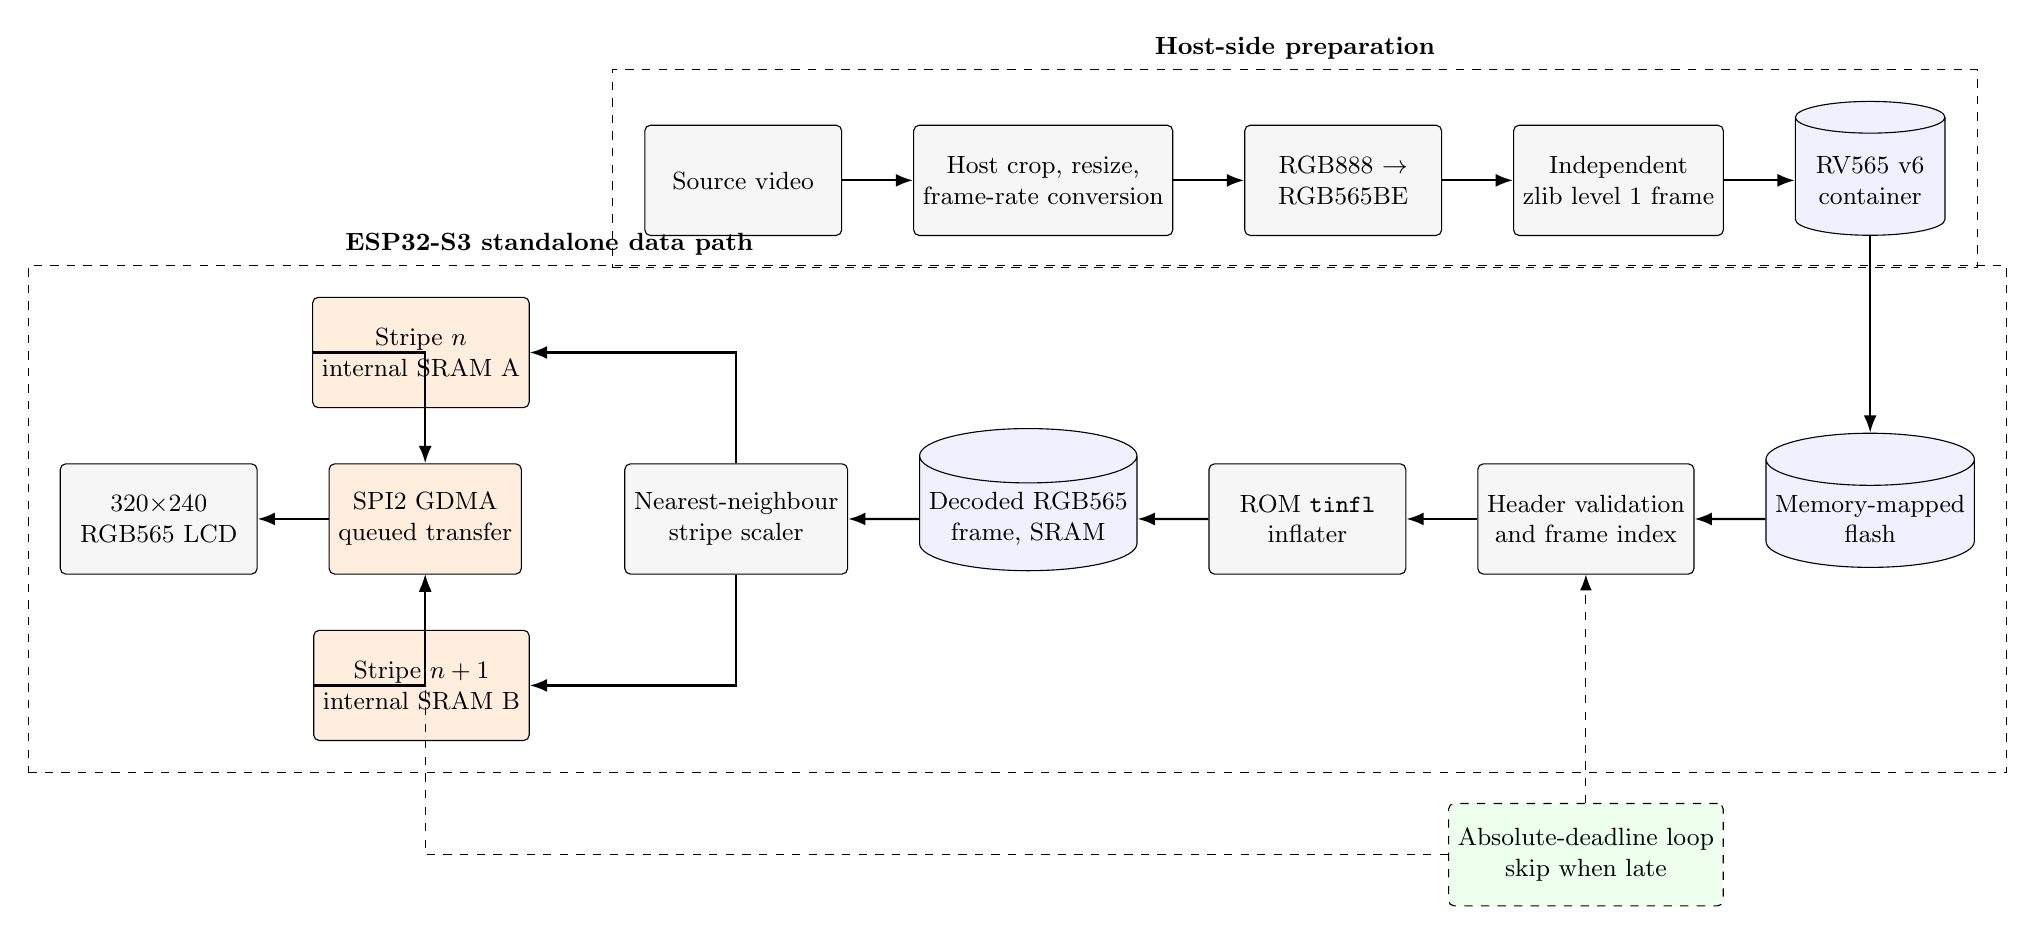
\begin{tikzpicture}[
  font=\small,
  node distance=7mm and 9mm,
  block/.style={draw, rounded corners=2pt, minimum height=14mm,
                minimum width=25mm, align=center, fill=gray!7},
  store/.style={draw, cylinder, shape border rotate=90, aspect=0.25,
                minimum height=17mm, minimum width=19mm, align=center,
                fill=blue!6},
  fast/.style={draw, rounded corners=2pt, minimum height=14mm,
               minimum width=24mm, align=center, fill=orange!13},
  control/.style={draw, dashed, rounded corners=2pt, minimum height=13mm,
                  minimum width=25mm, align=center, fill=green!7},
  flow/.style={-{Latex[length=2.2mm]}, thick},
  ctl/.style={-{Latex[length=2mm]}, dashed}
]
  \node[block] (source) {Source video};
  \node[block, right=of source] (host) {Host crop, resize,\\frame-rate conversion};
  \node[block, right=of host] (rgb) {RGB888 $\rightarrow$\\RGB565BE};
  \node[block, right=of rgb] (deflate) {Independent\\zlib level 1 frame};
  \node[store, right=of deflate] (container) {\system{} v6\\container};

  \node[store, below=25mm of container] (storage) {Memory-mapped\\flash};
  \node[block, left=of storage] (parser) {Header validation\\and frame index};
  \node[block, left=of parser] (inflate) {ROM \texttt{tinfl}\\inflater};
  \node[store, left=of inflate] (frame) {Decoded RGB565\\frame, SRAM};
  \node[block, left=of frame] (scale) {Nearest-neighbour\\stripe scaler};
  \node[fast, above left=7mm and 12mm of scale] (stripea)
       {Stripe $n$\\internal SRAM A};
  \node[fast, below left=7mm and 12mm of scale] (stripeb)
       {Stripe $n+1$\\internal SRAM B};
  \node[fast, left=13mm of scale] (dma) {SPI2 GDMA\\queued transfer};
  \node[block, left=of dma] (lcd) {320$\times$240\\RGB565 LCD};

  \node[control, below=29mm of parser] (scheduler) {Absolute-deadline loop\\skip when late};

  \draw[flow] (source) -- (host);
  \draw[flow] (host) -- (rgb);
  \draw[flow] (rgb) -- (deflate);
  \draw[flow] (deflate) -- (container);
  \draw[flow] (container) -- (storage);
  \draw[flow] (storage) -- (parser);
  \draw[flow] (parser) -- (inflate);
  \draw[flow] (inflate) -- (frame);
  \draw[flow] (frame) -- (scale);
  \draw[flow] (scale.north) |- (stripea.east);
  \draw[flow] (scale.south) |- (stripeb.east);
  \draw[flow] (stripea.west) -| (dma.north);
  \draw[flow] (stripeb.west) -| (dma.south);
  \draw[flow] (dma) -- (lcd);
  \draw[ctl] (scheduler) -- (parser);
  \draw[ctl] (scheduler.west) -| (dma.south);

  \node[draw, dashed, fit=(source)(host)(rgb)(deflate)(container),
        label=above:{\bfseries Host-side preparation}, inner sep=4mm] {};
  \node[draw, dashed, fit=(storage)(parser)(inflate)(frame)(scale)(stripea)(stripeb)(dma)(lcd),
        label=above left:{\bfseries ESP32-S3 standalone data path}, inner sep=4mm] {};
\end{tikzpicture}}
\caption{The \system{} standalone architecture.  Frame independence permits
indexed seeking and local recovery.  Alternating DMA-capable stripes allow CPU
scaling to overlap display transfer.  Dashed arrows carry scheduling.  The
OreoOS integration replaces the lower path with the serial stages of
Figure~\ref{fig:timeline}.}
\label{fig:architecture}
\end{figure*}

Figure~\ref{fig:hardware-platform} documents the hardware boundary used by the
measurements; the schematics are generated from KiCad~\cite{kicad} sources
in the repository~\cite{bhattacharya2026oreo}.  The first panel isolates the LCD clock, data, command/data,
reset, chip-select, and backlight paths.  The second places that display
beside the DevKit's flash/PSRAM configuration, USB connection, active-low
controls, and the header reserved for future input-latency tests.

\begin{figure*}[!tp]
\centering
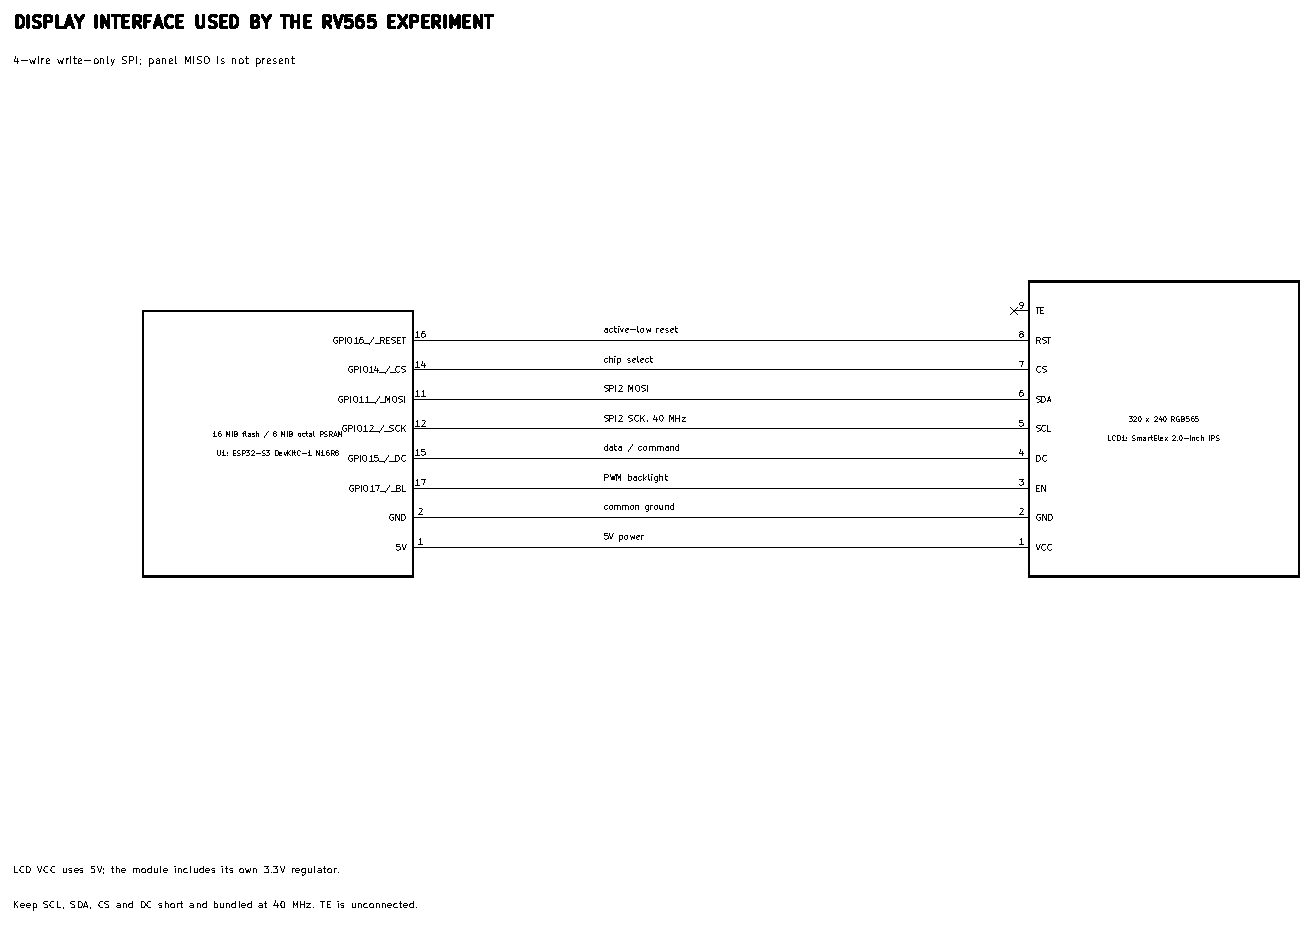
\includegraphics[width=0.94\textwidth]{figures/lcd_interface.pdf}
\\[-1mm]\textbf{(a)} LCD connection and signal path
\\[2mm]
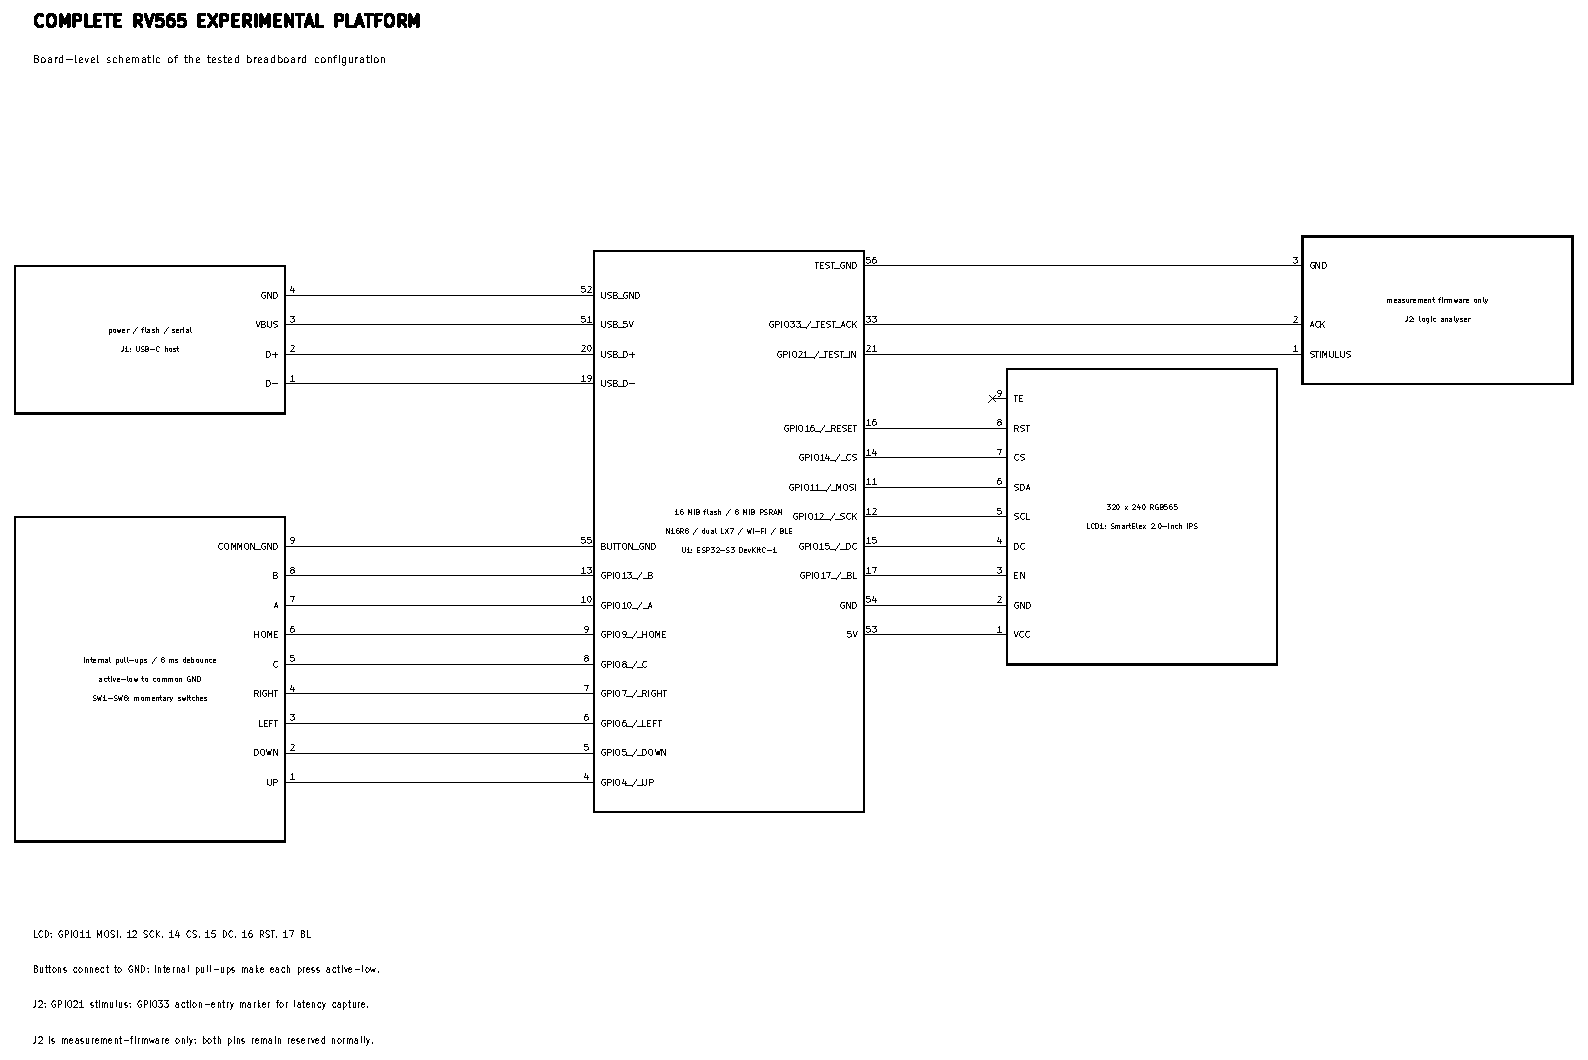
\includegraphics[width=0.94\textwidth]{figures/experimental_platform.pdf}
\\[-1mm]\textbf{(b)} Complete experimental circuit
\caption{Board-level schematics of the \system{} test platform.  Panel (a)
shows the 40~MHz write-only ST7789 interface.  Panel (b) shows the complete
video and interaction test path; GPIO21 and GPIO33 are reserved for stimulus
and acknowledgement markers in future input-latency firmware.}
\label{fig:hardware-platform}
\end{figure*}

\subsection{Container format}
\label{sec:container}

A \system{} v6 file begins with a 12-byte header containing a magic
identifier, format version, source width and height, frame rate, flags, and
frame count.  Each subsequent frame is stored as a little-endian 32-bit
compressed length followed by one zlib-wrapped Deflate payload.  Successful
inflation produces exactly $w\times h\times2$ bytes in RGB565 big-endian
order (Table~\ref{tab:format}).  The flags byte is currently zero.

\begin{table}[t]
\centering
\caption{\system{} v6 file layout. Multi-byte integers are little-endian;
decoded pixels are RGB565 big-endian.}
\label{tab:format}
\resizebox{\columnwidth}{!}{%
\begin{tabular}{rll}
\toprule
Offset & Size & Field \\
\midrule
0 & 3 & Magic, \texttt{RV5} \\
3 & 1 & Version, \texttt{6} \\
4 & 2 & Source width \\
6 & 2 & Source height \\
8 & 1 & Frame rate \\
9 & 1 & Flags (zero) \\
10 & 2 & Frame count \\
12 & 4 & Compressed length, frame 0 \\
16 & variable & zlib/Deflate payload, frame 0 \\
$\cdots$ & $\cdots$ & Repeated length and payload \\
\bottomrule
\end{tabular}
}
\end{table}

The length prefix permits a frame-offset table to be constructed in one scan.
Seeking then changes the compressed input position directly and does not
decode preceding frames.  Gallery builds the table lazily on the first seek;
the standalone firmware builds pointer and length tables (1,920~bytes for 240
frames) when the clip is opened.  Because lengths are known before any
payload is decoded, they also predict decode cost
(Section~\ref{sec:model}).

\subsection{Validation and failure recovery}
\label{sec:validation}

Media is checked at two boundaries.  Before transfer, the host ingest tool
decodes every compressed frame and verifies the magic, version, dimensions,
frame rate, frame count, exact RGB565 output length, complete payload
coverage, and absence of trailing data.  It then compares the encoded
artifact---not the source file---with both a media budget and the free space
reported by the badge.  An interrupted or malformed conversion is consequently
rejected before it can become Gallery input.

Device validation is repeated because stored media cannot be assumed to remain
trusted.  Dimensions must fit the 320$\times$240 panel, frame rate is limited
to 1--30~FPS, and frame count and compressed lengths must be nonzero and fit
the file and the allocated input buffer.  The standalone firmware
additionally rejects truncated tables and trailing bytes.  Inflation succeeds
only when it produces exactly $2wh$ bytes, so a partial decode is never
presented as a new frame.  Gallery currently fails closed when retrying the
frame after a rewind also fails.  Independence would permit a future policy
to skip a corrupt payload and resume at the next valid boundary; that policy
is not implemented.

\subsection{Host encoding}

The encoder (\texttt{tools/encode\_video\_benchmark.py}
in~\cite{bhattacharya2026oreo}) uses FFmpeg~\cite{ffmpeg} to resample the
source to the target frame rate, resize it with a Lanczos
filter~\cite{duchon1979lanczos} while preserving aspect ratio, crop to the
target dimensions, and convert to RGB565BE (Eq.~\eqref{eq:pixel}).  Every
frame is then compressed separately into a zlib stream~\cite{deutsch1996zlib}
at level~1, the fastest setting.  Encoder complexity is
thus irrelevant to device timing, and the level is a deliberate choice of
fast compression rather than minimum size (Section~\ref{sec:independence}).

\subsection{Native decode and stripe pipeline}

The standalone decoder (\texttt{experiments/video\_dma}
in~\cite{bhattacharya2026oreo}) reuses all large allocations, which are made
with ESP-IDF's capability-based allocator so that buffers can be restricted
to DMA-capable internal memory~\cite{espressif2026memalloc}.  It inflates one
independent payload directly from memory-mapped flash into the decoded frame
buffer, then scales output rows into one of two internal-memory stripes of
24 rows each, ten stripes per frame.  The chip select is held asserted across
the panel's RAMWR command and all stripes.  The first stripe is scaled and
queued as an SPI transaction serviced by GDMA~\cite{espressif2026spi,espressif2024trm};
while it is transferred, the CPU fills the other stripe; a wait for the
completed transaction precedes reuse of a buffer, after which the roles
alternate.  Measured work is therefore

\begin{equation}
T_{work}=T_{inflate}+T_{lcd},\qquad
T_{lcd}\approx T_{wire}+T_{scale}^{(1)}+\epsilon,
\label{eq:work}
\end{equation}

where $T_{wire}$ is the SPI wire time, $T_{scale}^{(1)}$ the unoverlapped
first stripe, and $\epsilon$ command and transaction overhead.  The remaining
nine stripes are scaled under DMA.  For a 320$\times$240 RGB565 frame on a
40~MHz single-lane bus,

\begin{equation}
T_{wire}=\frac{320\cdot240\cdot16\ \text{bit}}{40\ \text{MHz}}=30.72\ \text{ms},
\label{eq:wire}
\end{equation}

which bounds full-screen presentation at 32.55~FPS regardless of decoding.
Playback meets its target only when the upper tail of $T_{work}$, not merely
the mean, is below the period; the evaluation reports percentiles and the
worst observed value.

\subsection{OreoOS integration}

Gallery owns playback policy; at the measured revision, firmware owns only
inflation.  For each frame, Gallery reads one length-prefixed payload from the
filesystem into a reused compressed buffer and passes memoryviews of that
buffer and a reused RGB565 frame buffer to the firmware-resident
\texttt{\_oreo\_rv565} module, a MicroPython user C
module~\cite{micropython} (\texttt{firmware/usermods/oreo\_rv565}
in~\cite{bhattacharya2026oreo}).  That module calls
\texttt{tinfl}~\cite{miniz}, validates
the exact decoded length, and returns without constructing a temporary Python
\texttt{bytes} object or a Python-managed Deflate stream.  A separate native
Gallery routine then scales the frame into OreoOS's 153,600-byte framebuffer;
Python draws a playback overlay; and the display driver presents the frame
with blocking SPI writes in four 38,400-byte chunks separated by 200~$\mu$s
pauses, which smooth supply current on the badge.  Because the MicroPython
heap resides in PSRAM on this board, the compressed buffer, decoded frame,
and framebuffer are all in external RAM.  The stages are strictly serial
(Figure~\ref{fig:timeline}).

\subsection{Scheduling and interaction semantics}

For a clip rate $f$, the period is $P=1/f$ and the nominal deadline of frame
$i$ is

\begin{equation}
d_i=t_0+iP.
\label{eq:deadline}
\end{equation}

The standalone player advances the absolute deadline of
Eq.~\eqref{eq:deadline} after every transfer
and waits for the remainder of the period.  If the clock is more than one
period late, it advances both the deadline and frame index until they again
describe a future presentation; skipped frames are counted as drops and are
never decoded merely to catch up.

Gallery applies a bounded-work rule at the OS boundary instead: no more than
one frame is decoded per update tick, and accumulated delay beyond one period
is discarded rather than converted into a burst of work.  Gallery therefore
does not skip source frames when it falls behind; playback slows instead.
This bounds the time before the next input poll and makes slower playback
preferable to an unresponsive interface.

Each active-low button registers rising- and falling-edge interrupts whose
handlers only set preallocated flags; an 8~ms software debounce is applied
when the OS loop polls them.  MicroPython runs pin handlers as scheduled
(soft) callbacks unless a hard interrupt is requested~\cite{micropython2026pin},
and OreoOS uses the default, so they execute after the current native call
returns
and sample the pin level at that time rather than at the edge.  Whether a tap
shorter than a native frame operation is retained therefore depends on its
timing, and we make no input-latency or retention claim.

\section{Evaluation}
\label{sec:evaluation}

\begin{table}[t]
\centering
\caption{Evaluated configuration.  Revisions identify the commits whose
source files match the SHA-256 digests recorded with each measurement.}
\label{tab:platform}
\begin{tabular}{@{}>{\raggedright\arraybackslash}p{0.30\columnwidth}%
                >{\raggedright\arraybackslash}p{0.63\columnwidth}@{}}
\toprule
Parameter & Value \\
\midrule
Board & ESP32-S3-DevKitC-1 N16R8 \\
Processor & Dual-core Xtensa LX7, 240~MHz (configured) \\
Memory & 16~MiB flash, 8~MiB octal PSRAM \\
Display & ST7789, 320$\times$240, RGB565, 4-wire SPI \\
SPI clock & 40~MHz (driver-reported) \\
Standalone & ESP-IDF v5.5.1; source rev.\ \texttt{411f8f2}; PSRAM allocator disabled \\
Integrated & MicroPython v1.28.0 on ESP-IDF; Gallery rev.\ \texttt{dcca17b}; module rev.\ \texttt{de149c4} \\
Clip & 240 frames (10~s), 180$\times$135, 24~FPS \\
Container & 4,271,634 bytes (4.074~MiB) \\
\bottomrule
\end{tabular}
\end{table}

\subsection{Measurement methodology}

Timing uses the ESP32-S3 monotonic microsecond timer.  In the standalone
firmware, frame work begins immediately before inflation and ends when the
final queued LCD transaction completes; inflation, cumulative stripe scaling,
cumulative DMA wait, and the complete LCD phase are timed separately.  In
Gallery, frame work begins at the update tick that decodes the frame and ends
after the display flush; filesystem read, inflation, scaling, total drawing,
and presentation are timed separately, and the residual is attributed to the
OS loop and interpreter.  Displayed FPS is completed presentations divided by
wall time.  A deadline miss is frame work exceeding the period.

The standalone experiment uses a two-second, 48-frame warm-up and a
30-second, 720-frame timed window.  Ten independently reset runs provide 7,200
frame samples, covering every source frame 30 times.  Frame percentiles use
the pooled empirical distribution with linear interpolation between order
statistics (Hyndman and Fan's type~7~\cite{hyndman1996sample}); run-level
aggregates use two-sided 95\% Student-$t$ intervals~\cite{student1908probable}.
Linear models are ordinary least-squares fits, reported with Pearson's $r$.  Per-frame records are retained in RAM and printed
only after the timed window, so serial output does not enter the reported
latency.  Internal and external heap state is sampled at boot, after the clip
is opened, before playback, and after the timed window.  The integrated
experiment uses a 48-frame warm-up and one 720-frame window in the unmodified
OreoOS Gallery loop with the same media file.

Every result is tied to the SHA-256 digests of the application image,
media, build configuration, and relevant source files, and to the raw serial
log and per-frame CSV it was computed from.  A collector rejects any capture
whose numbered frame sequence is incomplete, and the aggregator refuses to
pool runs whose artifact hashes differ.  The collectors, aggregator, and the
script that derives every value in
Sections~\ref{sec:bus}--\ref{sec:gap} (\texttt{tools/analyze\_rv565\_paper.py})
are part of the released repository~\cite{bhattacharya2026oreo}.
Table~\ref{tab:platform} lists the evaluated configuration and the commits
whose sources match the recorded digests.

\subsection{Results}
\label{sec:standalone-results}

\begin{table*}[!t]
\centering
\caption{Measured \system{} v6 frame work.  Both rows play the same 4.074~MiB
file.  Integrated playback does not skip frames when late, so drops are not
applicable (n/a).}
\label{tab:results}
\resizebox{\textwidth}{!}{%
\begin{tabular}{lccccccccc}
\toprule
Path & Frames & FPS & Drops & Misses & Mean (ms) & p50 (ms) & p95 (ms) & p99 (ms) & Max (ms) \\
\midrule
Standalone: inflate + DMA stripes & 7,200 & 24.004 & 0 & 0 & 38.411 & 38.552 & 39.690 & 40.206 & 40.346 \\
OreoOS Gallery + firmware inflate & 720 & 14.093 & n/a & 720 & 69.212 & 69.535 & 76.988 & 78.938 & 79.442 \\
\bottomrule
\end{tabular}
}
\end{table*}

Table~\ref{tab:results} reports both paths.  The standalone path meets every
41.667~ms deadline; its worst frame leaves 1.321~ms of slack.  Run-level
variation is negligible: the 95\% interval on mean frame work is
38.4106--38.4107~ms, and the run-level p99 ranges over 1~$\mu$s.  Paced FPS
is fixed by the deadline loop, so tail margin and the miss count are the
informative quantities.

The integrated path misses all 720 deadlines and presents 14.093~FPS.
Because Gallery slows rather than skips, the clip plays at 0.587$\times$ real
time.

\begin{figure*}[t]
\centering
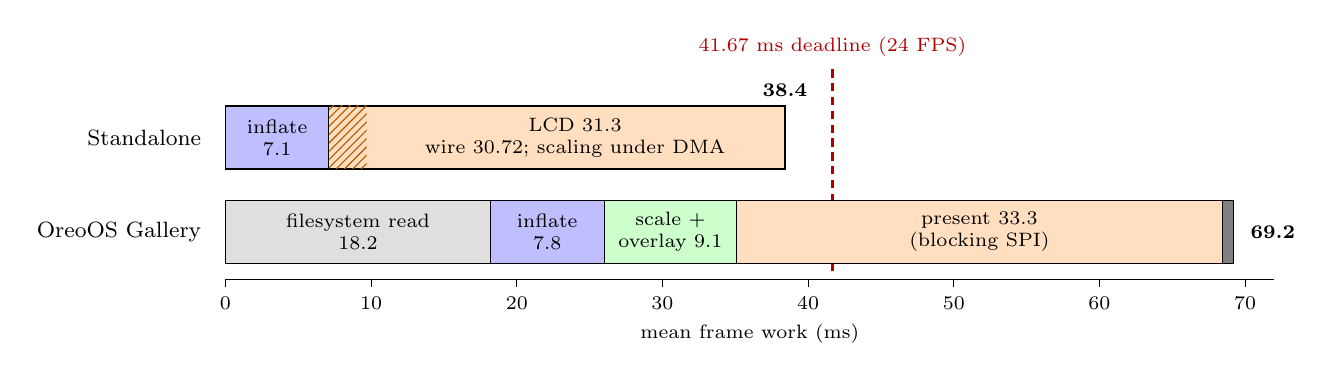
\begin{tikzpicture}[x=1.85mm, y=1mm, font=\scriptsize]
  % Deadline
  \draw[red!70!black, densely dashed, thick] (41.667,-1) -- (41.667,25)
    node[above] {41.67 ms deadline (24 FPS)};
  % Standalone
  \node[anchor=east, align=right, font=\footnotesize] at (-1,16) {Standalone};
  \draw[fill=blue!25] (0,12) rectangle (7.097,20);
  \node[align=center] at (3.55,16) {inflate\\7.1};
  \draw[fill=orange!25] (7.097,12) rectangle (38.409,20);
  \fill[pattern=north east lines, pattern color=orange!70!black]
    (7.097,12) rectangle (9.696,20);
  \node[align=center] at (24,16) {LCD 31.3\\wire 30.72; scaling under DMA};
  \node[above] at (38.409,20) {\textbf{38.4}};
  % Gallery
  \node[anchor=east, align=right, font=\footnotesize] at (-1,4) {OreoOS Gallery};
  \draw[fill=gray!25] (0,0) rectangle (18.193,8);
  \node[align=center] at (9.1,4) {filesystem read\\18.2};
  \draw[fill=blue!25] (18.193,0) rectangle (25.991,8);
  \node[align=center] at (22.09,4) {inflate\\7.8};
  \draw[fill=green!20] (25.991,0) rectangle (35.107,8);
  \node[align=center] at (30.55,4) {scale +\\overlay 9.1};
  \draw[fill=orange!25] (35.107,0) rectangle (68.415,8);
  \node[align=center] at (51.76,4) {present 33.3\\(blocking SPI)};
  \draw[fill=black!50] (68.415,0) rectangle (69.212,8);
  \node[anchor=west] at (69.7,4) {\textbf{69.2}};
  % Axis
  \draw (0,-2) -- (72,-2);
  \foreach \t in {0,10,20,30,40,50,60,70} {
    \draw (\t,-2) -- (\t,-3); \node[below] at (\t,-3) {\t};
  }
  \node[below] at (36,-6.5) {mean frame work (ms)};
\end{tikzpicture}
\caption{Mean per-frame critical path, drawn to scale from the measured stage
times.  The standalone path overlaps scaling (hatched, first stripe only on
the critical path) with DMA and is bounded by the SPI wire time; the
integrated path executes every stage serially.  The dark segment is OS and
interpreter residual (0.80~ms).}
\label{fig:timeline}
\end{figure*}

\subsection{The standalone path is bus-bound}
\label{sec:bus}

Mean $T_{lcd}$ is 31.312~ms against the 30.72~ms wire time of
Eq.~\eqref{eq:wire}: the display transfer runs at 98.1\% of the bus bound.
Within it, the CPU spends 2.599~ms scaling and 28.470~ms waiting for DMA, so
it is idle for 90.9\% of the transfer.  Mean inflation is 7.097~ms (p99
8.889~ms), and Eq.~\eqref{eq:work} accounts for the measured mean work to
within 2~$\mu$s.  Both quantities are tightly distributed: $T_{lcd}$ varies by
only 12~$\mu$s between p50 and maximum, so nearly all tail variation comes
from content-dependent inflation.

The idle time is the next opportunity.  Inflating frame $k+1$ while frame $k$
is transferred would need a second 48,600-byte decoded buffer, which fits in
the 241.2~KiB of internal memory that remained free (Table~\ref{tab:resources}).
It would add about 7.1~ms of CPU work inside a 28.5~ms idle window, bounding
the period by $T_{lcd}$ alone: approximately 31.9~FPS, against the 32.55~FPS
wire-time limit.  This is a projection from the measured components, not a
measured result.

\subsection{Decode cost is predictable from the container}
\label{sec:model}

Compressed frame sizes range from 6,558 to 25,682~bytes (mean 17,794).
Across all 7,200 standalone frames, inflation time is linear in the stored
length $L$:

\begin{equation}
T_{inflate}\approx 3.117\ \text{ms} + 0.2236\ \mu\text{s/byte}\times L,
\label{eq:inflate}
\end{equation}

with $r=0.978$ ($r^2=0.957$).  The intercept reflects the fixed cost of
producing 48,600 output bytes; the slope reflects symbol decoding.  Fitting
on even-numbered source frames and testing on odd-numbered frames gives a
mean absolute error of 0.138~ms and a maximum error of 0.538~ms.  For the
largest frame the model predicts 8.86~ms; the slowest observed instance of
that frame took 8.94~ms.

Because $L$ is stored in the container, worst-case decode time is known when
a file is ingested, before it is played.  Combined with the nearly constant
$T_{lcd}$, a host tool can decide whether a clip is schedulable at a given
rate and resolution from metadata alone, or re-encode it until it is.  This
property follows from independent, single-codec frames; it would not hold for
formats whose decode cost depends on reference state.

\subsection{The cost of frame independence}
\label{sec:independence}

The container occupies 4,271,634~bytes, against 11,664,012~bytes for the same
240 frames stored raw: a ratio of 2.73$\times$.  To measure what independence
gives up, we decoded the evaluated container losslessly on the host and
recompressed the identical RGB565 frames under alternative organisations
(Table~\ref{tab:independence}).  Recompressing each frame at level~1
reproduces all 240 payloads byte for byte, confirming the setup.

\begin{table}[t]
\centering
\caption{Deflate payload bytes for the evaluated 240 frames under alternative
organisations, relative to the shipped independent level-1 payloads.}
\label{tab:independence}
\resizebox{\columnwidth}{!}{%
\begin{tabular}{lrr}
\toprule
Organisation & Bytes & Relative \\
\midrule
Independent frames, level 1 (shipped) & 4,270,662 & 1.000 \\
Single stream, level 1 & 4,244,946 & 0.994 \\
Independent frames, level 6 & 3,554,817 & 0.832 \\
Independent frames, level 9 & 3,550,852 & 0.831 \\
Single stream, level 9 & 3,489,148 & 0.817 \\
XOR with previous frame, level 1 & 5,275,672 & 1.235 \\
\bottomrule
\end{tabular}
}
\end{table}

Compressing all frames as one stream saves only 0.60\% at level~1 and 1.74\%
at level~9, as Eq.~\eqref{eq:window} predicts for a 48,600-byte frame: no
co-located pixel of the previous frame is reachable.  The compression level
matters about ten times more than independence: level~6 would shrink the
payload by 16.8\%.  Its effect on device inflation time was not measured, so
level~1 remains the evaluated configuration.  A naive XOR delta against the
previous frame is 23.5\% larger: in this clip, XOR residuals compress worse
than the frames themselves.  Exploiting temporal redundancy would therefore
require motion compensation, which is exactly the decoder state that
\system{} avoids.

\subsection{Anatomy of the integration gap}
\label{sec:gap}

Table~\ref{tab:gallery} decomposes integrated frame work.  The interpreter
and OS loop account for only 0.80~ms on average (p99 1.37~ms).  The gap to
the standalone path comes from three structural differences.

\begin{table}[t]
\centering
\caption{Integrated Gallery stage times (720 frames).  Overlay is drawing
time other than scaling; the residual is OS loop and interpreter work.}
\label{tab:gallery}
\small
\setlength{\tabcolsep}{4pt}
\begin{tabular}{lrrr}
\toprule
Stage & Mean (ms) & p99 (ms) & Max (ms) \\
\midrule
Filesystem read & 18.193 & 25.934 & 26.748 \\
Inflation & 7.798 & 9.541 & 9.638 \\
Scaling (native) & 7.650 & 8.204 & 8.832 \\
Overlay & 1.466 & 2.151 & 7.003 \\
Presentation & 33.308 & 33.924 & 34.361 \\
OS residual & 0.797 & 1.367 & 5.450 \\
\midrule
Frame work & 69.212 & 78.938 & 79.442 \\
\bottomrule
\end{tabular}
\end{table}

\paragraph{Filesystem input.}  Read time is linear in payload length
(1.111~ms + 0.960~$\mu$s/byte, $r=0.984$), an effective throughput of about
1.0~MB/s.  Extrapolated to an uncompressed 48,600-byte frame, the read alone
would take about 47.8~ms, beyond the 41.7~ms period.  On this path, Deflate is
therefore not merely a storage optimisation: it trades 7.8~ms of inflation for
roughly 29.6~ms of avoided reads.  The standalone path avoids the cost
entirely by reading memory-mapped flash.

\paragraph{Memory placement.}  Integrated inflation has nearly the same
per-byte cost as the standalone path (0.2109 versus 0.2236~$\mu$s/byte) but a
0.93~ms larger intercept (4.046 versus 3.117~ms), consistent with writing the
48,600-byte output to PSRAM instead of internal SRAM.  Scaling takes 7.650~ms
against 2.599~ms; it writes a complete 153,600-byte framebuffer in PSRAM
rather than SRAM stripes, though the two kernels also differ, so the 2.9$\times$
ratio is not attributed to memory placement alone.

\paragraph{Serialized presentation.}  Presentation costs 33.308~ms, 2.59~ms
above the wire time, of which 0.6~ms are the deliberate inter-chunk pauses.
Unlike the standalone path, no other stage runs during it.

These results determine the next step.  Removing the filesystem read alone
would leave about 51.0~ms of serial work, still above the period.  Meeting
24~FPS inside OreoOS requires the standalone structure---memory-resident
input, SRAM stripes, and scaling overlapped with DMA---to become a single
firmware operation invoked once per frame by Gallery.

\begin{table}[t]
\centering
\caption{Measured standalone memory use (internal SRAM; identical in all ten
runs).}
\label{tab:resources}
\resizebox{\columnwidth}{!}{%
\begin{tabular}{lrrrr}
\toprule
Allocation & SRAM & PSRAM & Drift & Minimum free \\
\midrule
Native DMA path & 79.9 KiB & 0 KiB & 1.3 KiB & 241.2 KiB \\
\bottomrule
\end{tabular}
}
\end{table}

\subsection{Memory}

Table~\ref{tab:resources} reports the standalone path's 81,816-byte
(79.9~KiB) incremental allocation: the 48,600-byte decoded frame, two
15,360-byte stripes, the frame tables, and allocator overhead.  It excludes
the 23,040-byte (22.5~KiB) per-frame measurement array.  The 1.3~KiB drift
between the pre-playback and final samples includes SPI driver
initialisation, which occurs after the pre-playback sample; it is identical
in every run, so playback does not grow the heap.  Integrated memory was not
sampled during playback.  By construction, Gallery allocates a 48,600-byte
frame buffer and a 49,624-byte compressed buffer in addition to the
153,600-byte framebuffer that OreoOS already holds, all in PSRAM.

\section{Limitations and Threats to Validity}

The evaluation uses one ten-second clip, one board, and one resolution and
rate.  The linear decode model and the independence measurements are
therefore properties of this workload; content with different statistics may
change the coefficients, though Eq.~\eqref{eq:window} does not depend on
content.  The decode model is fitted and tested on the same clip, split by
frame.  We report no image-quality metric: loss arises only from resampling
and RGB565 quantisation, which an evaluation must measure against a fixed
resized RGB888 reference using PSNR and SSIM~\cite{wang2004image}.

No codec baseline is reported.  A comparison with MJPEG or with Espressif's
player~\cite{espressif2026player} must hold decoded dimensions, rate, clip
range, and quality constant, and must consider the complete resource envelope
rather than size or FPS alone.  No ablation was run; the integrated row
differs from the standalone row in input path, memory placement, scaling
kernel, presentation, and the presence of the OS, and
Section~\ref{sec:gap} separates these by stage timing rather than by
controlled removal.  Input latency was not measured.  The CPU clock is the
configured value, not a measurement.  The standalone runs were captured from a
working tree whose benchmark source and build defaults were committed as
\texttt{411f8f2} with matching hashes.

\system{} is currently silent, RGB565-specific, and intended for small
displays.  Future work includes the fused firmware playback path, overlapping
inflation with transfer, SD-card streaming, synchronised audio, a
schedulability check in the ingest tool based on Eq.~\eqref{eq:inflate},
quality-matched codec baselines, logic-analyser input-latency measurement, and
other processors and bus widths.

\section{Conclusion}

\system{} treats microcontroller video as one timed storage, memory,
decoding, scheduling, and display problem.  On an ESP32-S3, independent
display-native frames and double-buffered DMA stripes sustain 24.004~FPS
across 7,200 frames with zero misses, with the display transfer at 98.1\% of
the SPI wire-time bound.  Independent Deflate frames make decode cost a
linear function of stored length and, above $128\times128$ pixels, give up
almost no compression.  Inside a MicroPython operating system, moving
inflation into firmware is insufficient: the stage-resolved measurements
place the remaining cost in serialized filesystem input, external-memory
placement, and blocking presentation rather than in the interpreter, and
identify the single fused firmware operation that should come next.

\section*{Artifact Availability}

OreoOS, the \system{} encoders, firmware modules, standalone benchmark, paper
source, raw serial logs, per-frame data, artifact hashes, and the scripts
that produce every reported value are archived at
\url{https://doi.org/\artifactdoi} and developed at
\url{https://github.com/elixpo/oreo}~\cite{bhattacharya2026oreo}.

\begingroup
\fontsize{7pt}{7.4pt}\selectfont
\bibliographystyle{unsrt}
\bibliography{references}
\endgroup

\end{document}
